% Preamble -------------------------------------------------
\documentclass{beamer}
\usepackage[german]{babel}
\usepackage{bibentry}

\addbibresource{./library.bib}

\definecolor{grey538}{RGB}{240,240,240}

\newcommand*{\priority}[1]{\begin{tikzpicture}[scale=0.15]%
    \draw (0,0) circle (1);
    \fill[fill opacity=.4,fill=blue] (0,0) -- (90:1) arc (90:90-#1*3.6:1) -- cycle;
    \end{tikzpicture}}
% document body --------------------------------------------
\begin{document}

\maketitle

\begin{frame}
    \frametitle{Leitfragen der Sitzung}
    \begin{enumerate}
        \item Was gehört zur Programmatik politischer Parteien?
        \item Warum wertet man bevorzugt Wahlprogramme aus?
        \item Was kann man mit so einer Auswertung anfangen?
    \end{enumerate}
\end{frame}

\begin{frame}
    \frametitle{Was zählt zur Programmatik politischer Parteien?}
    \textbf{Pogrammatik einer Partei}
    \begin{itemize}
        \item Übersetzung gesellschaftl. Interessen in polit. Forderungen
    \end{itemize}

    \textbf{Programmarten}
    \begin{itemize}
        \item Grundsatzprogramm, Aktionsp., Kurzp., Wahlp.
        \item Unterschiede: Beständigkeit, Umfang, Addressat, Zweck
    \end{itemize}

    \begin{center}
        \footnotesize
        \begin{tabular}{*{3}{l}}
            \toprule
            \textbf{Parteiziel} & \textbf{Programmfunktion} & \textbf{Addressat} \\
            \midrule
            \multirow{2}{*}{Politikverwirklichung} & Praxisanleitung & Parlamentarier \& \\
            & Ideologieübersetzung & Minister \\
            \multirow{2}{*}{Stimmenmaximierung} & Werbung & \multirow{2}{*}{Wähler \& Medien} \\
            & Profilbildung & \\
            \multirow{2}{*}{Regierungsbeteiligung} & Operationsbasis & \multirow{2}{*}{andere Parteien} \\
            & Signalisierung & \\
            \multirow{2}{*}{Innerpart. Demokratie} & Integration & \multirow{2}{*}{Parteibasis} \\
            & Kontroll \& Legitimation & \\
            \bottomrule
        \end{tabular}
    \end{center}
\end{frame}

\begin{frame}
    \frametitle{Warum wertet man bevorzugt Wahlprogramme aus?}
    \begin{enumerate}
        \item \textbf{Aktualität}: Wahlp. ändern sich mit jeder Wahlperiode.
        \item \textbf{Verfügbarkeit}: Alle Parteien formulieren Wahlprogramme.
        \item \textbf{Querschnitt}: Wahlprogramme bedienen alle Parteiziele.
    \end{enumerate}

    \begin{center}
        \begin{tabular}{*{5}{l}}
            \toprule
            & \textbf{Grundsatz} & \textbf{Aktion} & \textbf{Kurz} & \textbf{Wahl} \\
            \midrule
            Politikverwirklichung & \priority{66} & \priority{100} & \priority{33} & \priority{66} \\
            Stimmenmaximierung & \priority{0} & \priority{0} & \priority{0} & \priority{66} \\
            Regierungsbeteiligung  & \priority{0} & \priority{66} & \priority{100} & \priority{66} \\
            Innerpart. Demokratie  & \priority{100} & \priority{0} & \priority{0} & \priority{66} \\
            \bottomrule
        \end{tabular}
    \end{center}
\end{frame}

\begin{frame}
    \frametitle{Was kann man mit so einer Auswertung anfangen?}
    \begin{itemize}
        \item Grundlage gehaltvoller empirisch-analytische Forschung
        \item Bspw. erhob das \href{https://manifesto-project.wzb.eu/}{Manifesto Projekt}
        \begin{itemize}
            \item seit 1945
            \item in über 50 Ländern
            \item Wahlprogramme von mehr als 1000 politischen Parteien.
        \end{itemize}
    \end{itemize}
    \begin{figure}
        \centering
        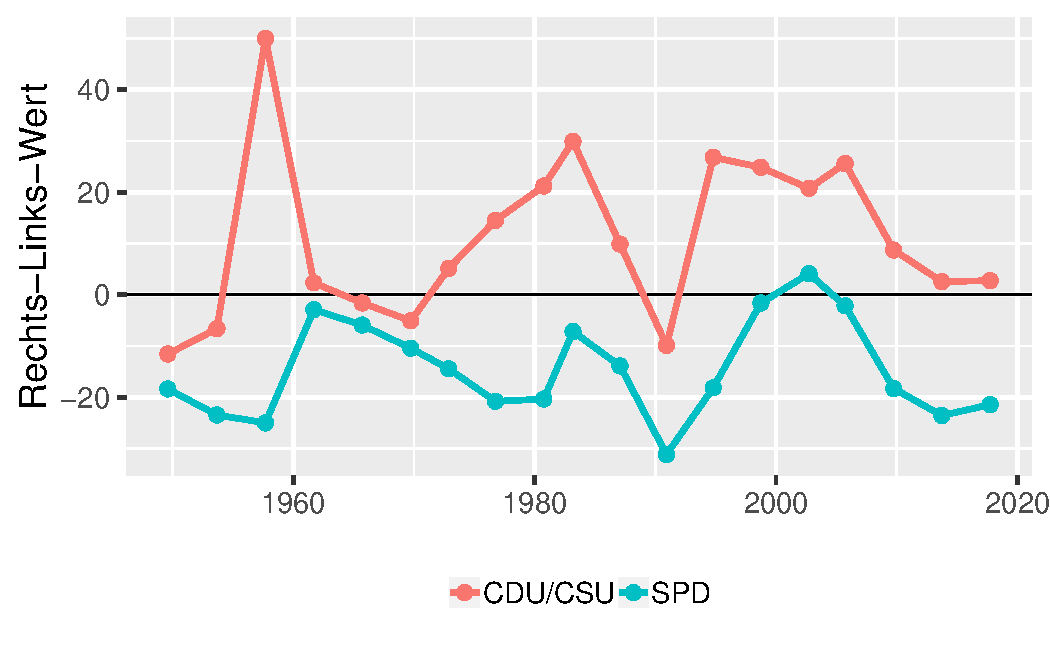
\includegraphics[scale = .4]{./centerPartiesDE.pdf}
    \end{figure}
\end{frame}
\end{document}
